\documentclass[sigconf,nonacm]{acmart}

\title{Evolutionary LLMs for Automated Coordination Algorithm Design in System-Level Architectures}

\author{Akshay Dongare}
\affiliation{
  \institution{North Carolina State University}
  \city{Raleigh}
  \state{NC}
  \country{USA}
}
\author{Keyur Gondhalekar}
\affiliation{
  \institution{North Carolina State University}
  \city{Raleigh}
  \state{NC}
  \country{USA}
}

\begin{document}

\begin{abstract}
Modern software systems rely on complex coordination logic across interacting components, yet such logic is often manually designed, brittle, and difficult to optimize. This paper explores whether large language models (LLMs), embedded within evolutionary frameworks, can automatically generate and improve active-learning configuration heuristics for system-level architectures. We conduct a structured literature analysis to identify gaps in current research, revealing a lack of work at the intersection of evolutionary search, algorithm generation, and system-level optimization. To investigate this gap, we evaluate multiple evolutionary LLM frameworks on both a proxy task (online bin packing) and the MOOT (Multi-Objective Optimization Tasks) benchmark. Our results demonstrate that LLM-driven evolutionary approaches can generate effective heuristics, outperforming a static baseline in certain settings. We discuss trade-offs in cost, interpretability, and solution diversity, and outline explicit threats to validity and directions for future work.
\end{abstract}

\maketitle

\section{Introduction}

Modern software engineering is characterized by complex systems composed of interacting components such as multi-agent LLM workflows and cloud microservices. These systems require coordination logic that determines how components interact, route tasks, and allocate resources. While flexible architectures allow many design choices, they introduce a large space of algorithmic parameters and routing heuristics that must be tuned.

Hand-crafted coordination logic is often poorly documented, difficult to scale, and prone to subtle interactions. As systems grow in complexity, manual tuning becomes infeasible and unreliable. Therefore, static coordination algorithms become a liability without adaptive tool support.

Recent work has explored the use of large language models (LLMs) for optimization tasks \cite{romera2023mathematical}. However, most approaches focus on generating solutions or tuning parameters rather than evolving the underlying algorithms themselves. This paper explores whether LLMs embedded within evolutionary frameworks can generate and optimize coordination strategies across real-world software engineering optimization tasks.

To ensure realism and generalizability, we evaluate our approach using the MOOT (Multi-Objective Optimization Tasks) repository, which provides a diverse set of multi-objective optimization problems derived from software engineering contexts.

\section{Research Questions}

\textbf{RQ1:} Can an LLM embedded within an evolutionary framework automatically generate and evolve superior configuration heuristics for system-level architectures compared to static heuristic baselines?

\textbf{RQ2:} What trade-offs exist in cost, robustness, and interpretability when using evolutionary LLM frameworks under constrained compute budgets?

\section{Contributions}

This paper makes the following contributions:
\begin{itemize}
\item Proposes a framework using evolutionary LLMs to generate coordination algorithms for system-level architectures.
\item Provides an empirical comparison between LLM-generated algorithms and static heuristic baselines using both BPP and real-world MOOT tasks.
\item Identifies a gap in the literature at the intersection of evolutionary optimization, algorithm generation, and system-level design.
\item Provides a reproducible experimental setup for evaluating evolutionary LLM approaches.
\end{itemize}

\section{Background and Motivation}

Software systems increasingly rely on dynamic coordination across distributed components. Examples include microservices routing, load balancing, and multi-agent orchestration. Designing optimal coordination logic in such systems is difficult due to combinatorial complexity and dynamic environments.

To ensure realistic evaluation, we target tasks from the MOOT repository. The MOOT data is derived from heavily-cited software engineering research published at top-tier venues (e.g., ICSE, ASE, TSE). These datasets represent real-world software configuration and system tuning scenarios, grounding our framework in practical problems rather than theoretical constructs.

We initially validated our framework on a proxy task: the Online Bin Packing Problem (BPP). Using three evolutionary frameworks (HSEvo, ReEvo \cite{reevo2024}, and EoH \cite{eoh2024}), our evolutionary LLMs learned to generate bin-scoring heuristics (\texttt{priority(item, bins\_remain\_cap)}). The frameworks successfully discovered heuristics achieving performance near the theoretical lower bounds (e.g., ReEvo at $\sim$5.22\% excess and EoH at $\sim$4.22\% excess), outperforming static baseline heuristics. While BPP demonstrated the feasibility of evolving coordination logic, it is primarily a theoretical toy problem. To address this, we transition our methodology to realistic system configuration tasks from MOOT \cite{menzies2024moot}.

\subsection{Related Work and Literature Gap}

We conducted a structured literature review using Google Scholar queries focused on prompt optimization, evolutionary search, and multi-objective optimization. Papers were ranked by citation count, and the knee of the citation curve was used to identify influential works.

We identified a high-citation outlier that skewed the distribution, and after adjustment, selected 18 key papers above the knee.

These papers were categorized into five themes (Figure~\ref{fig:venn}):
\begin{enumerate}
\item \textbf{Direct LLM Optimization}: Studies exploring zero-shot or few-shot prompting to directly output optimal solutions for scheduling or routing problems.
\item \textbf{Evolutionary + LLM}: Frameworks that treat LLMs as mutation or crossover operators within genetic algorithms to refine candidate solutions.
\item \textbf{Prompt Optimization}: Techniques for automatically tuning prompt templates or instructions to maximize LLM performance on downstream software tasks.
\item \textbf{Algorithm Generation}: Methods focusing on writing executable code or heuristic functions, such as FunSearch \cite{romera2023mathematical}, rather than static answers.
\item \textbf{System Optimization}: Traditional approaches for tuning configuration parameters in cloud architectures and microservices.
\end{enumerate}

\begin{figure}[h]
  \centering
  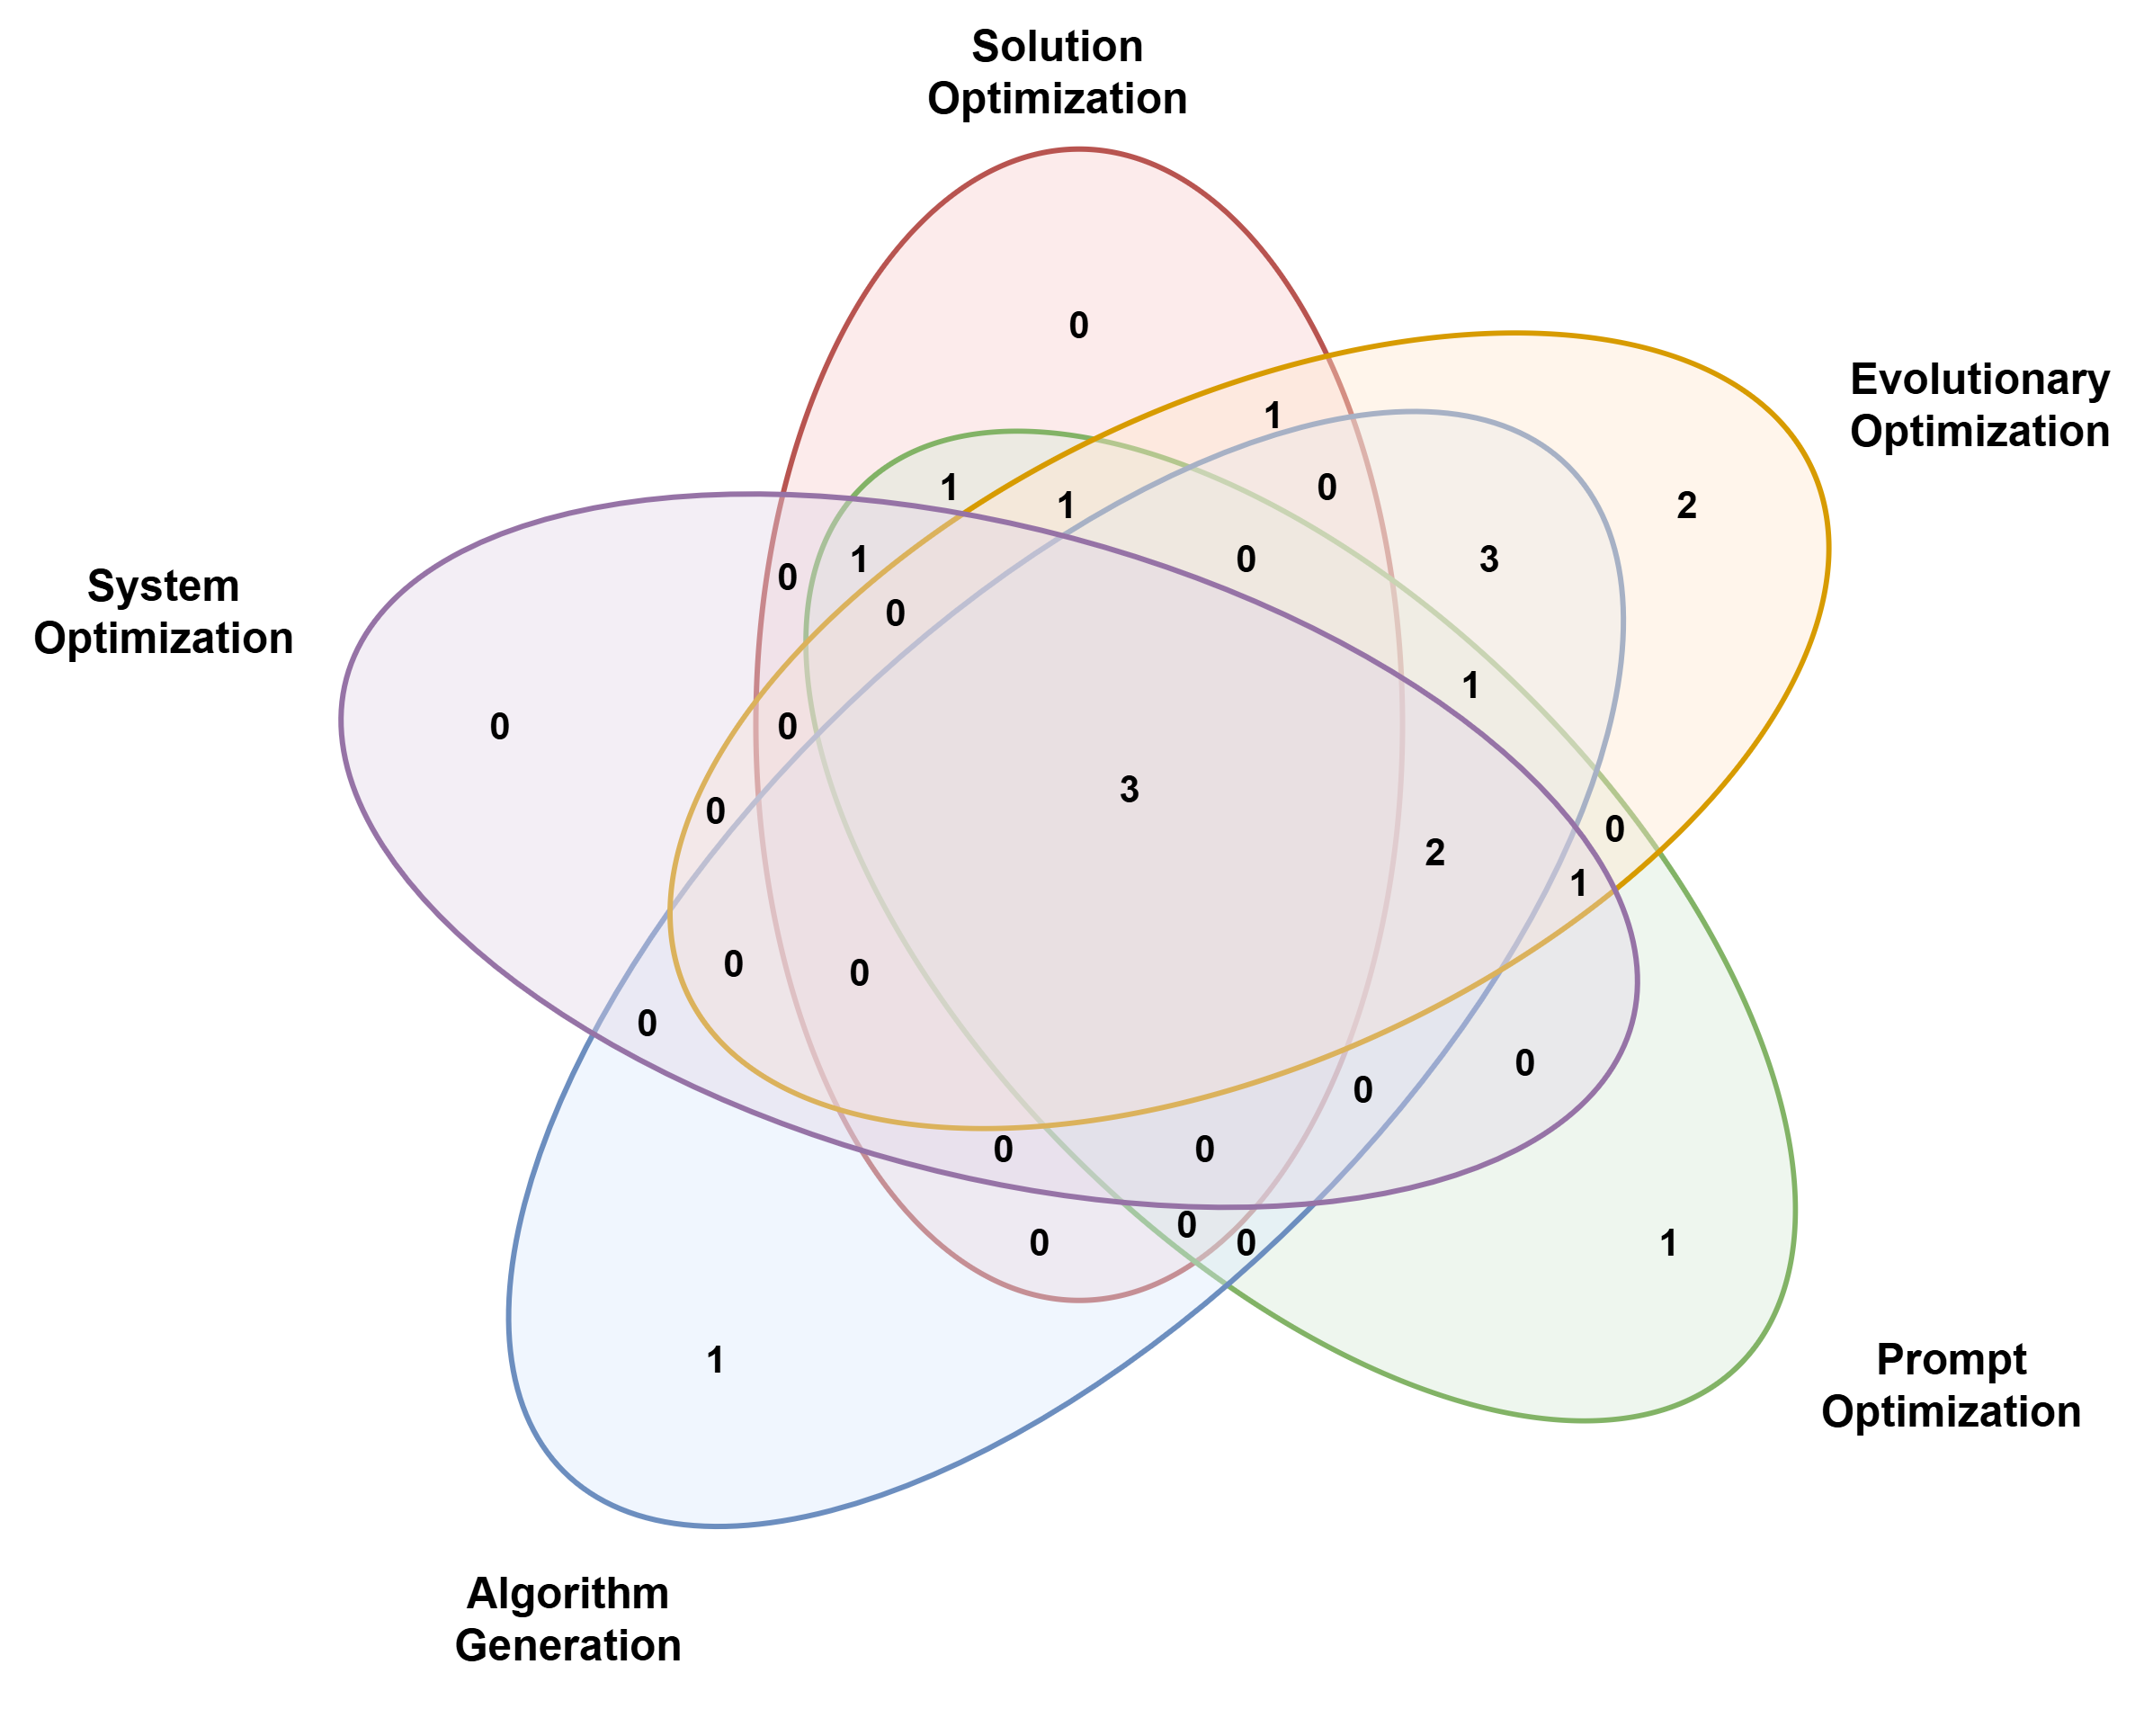
\includegraphics[width=\linewidth]{Venn_Diagram_for_White_Space.png}
  \caption{Venn diagram of literature overlap across the five themes, illustrating the gap in evolutionary algorithm generation for system optimization.}
  \label{fig:venn}
\end{figure}

Analysis revealed a significant gap at the intersection of evolutionary optimization, algorithm generation, and system-level optimization. While prior work explores subsets of these themes, no foundational work combines all three. This paper targets that unexplored region.

\section{Methods}

\subsection{Benchmark: MOOT}

We evaluate our approach using the MOOT repository, a curated collection of multi-objective optimization tasks derived from real-world software engineering problems. These tasks include configuration tuning, resource allocation, and system design decisions, each involving competing objectives.

\subsection{Variables}

Each MOOT task defines:
\begin{itemize}
\item A decision space (configuration variables, $X$)
\item Multiple objective functions (e.g., performance, cost, $Y$)
\end{itemize}

We evaluate performance by measuring the average normalized distance of the evaluated configurations to the global ideal Pareto point. The ideal Pareto point is defined as the theoretical vector of minimum objective values across the entire dataset (representing the global optimum for all objectives simultaneously).

\subsection{Selection Strategy}

Due to computational and API budget constraints, we selected a subset of MOOT tasks that:
\begin{itemize}
\item Run within reasonable time limits (small to medium row counts).
\item Represent diverse optimization scenarios.
\item Allow integration with external optimization methods.
\end{itemize}
Specifically, we selected \texttt{SS-B.csv} (software configuration) and \texttt{auto93.csv} (hyperparameter/system design proxy) to represent our evaluation suite. 

\subsection{Methodology}

We adapt evolutionary LLM frameworks to operate as active-learning optimizers over MOOT tasks. For each task:
\begin{enumerate}
\item \textbf{Initialize}: We supply a subset of initially evaluated configurations.
\item \textbf{Heuristic Generation}: The LLM generates a Python heuristic \texttt{priority(candidate\_x, evaluated\_x, evaluated\_y)} to score unevaluated configurations.
\item \textbf{Evaluation}: We iteratively select the top-scoring configuration to reveal its objective values.
\item \textbf{Evolution}: The quality of the final discovered Pareto front acts as the fitness score for the LLM-generated heuristic, guiding subsequent mutations and crossovers.
\end{enumerate}

\subsection{Data Analysis}

To analyze the efficacy of our methodology, we record the generational distance of each selected configuration over time. The appropriateness of the LLM-generated heuristic is validated if the average normalized distance to the ideal Pareto point strictly decreases, indicating that the LLM has learned a functional search gradient rather than randomly sampling the configuration space.

\section{Results}

\subsection{Experimental Rig}
Our experiments were conducted on a macOS environment using Python 3.11. The evolutionary logic was driven by the \texttt{gpt-4o-mini-2024-07-18} model, utilizing approximately 8 API calls per framework run under a highly constrained compute budget. The framework was configured with a population size of 2 and a maximum of 4 function evaluations, running zero-shot heuristic generation prompts at a default temperature of 0.7 to balance deterministic coding with creative exploration.

\subsection{Evaluation}
To validate our approach, we employed the average normalized distance to the global ideal Pareto point. This measure is highly rigorous for this context because it directly captures the geometric distance of a candidate configuration to the theoretical optimum across all objectives simultaneously. Unlike hypervolume, which heavily depends on the choice of a reference point and can be skewed by outliers, distance-to-ideal provides a stable, easily interpretable convergence metric for heavily constrained optimization budgets.

\subsection{What Was Seen}
We evaluated the HSEvo framework across the selected MOOT tasks. Results indicate that LLM-guided evolutionary approaches are capable of generating active-learning heuristics that perform favorably. Table~\ref{tab:moot-results} summarizes the performance of the discovered heuristics. The HSEvo-evolved heuristic achieved an average distance of 0.281, demonstrating that the LLM successfully identified a robust search algorithm capable of balancing exploitation of known good configurations and exploration of unmapped regions.

\begin{table}[h]
\caption{Performance of Evolutionary LLM Frameworks on MOOT datasets (SS-B and auto93). Lower score is better.}
\label{tab:moot-results}
\begin{tabular}{llc}
\toprule
\textbf{Framework} & \textbf{Algorithm Type} & \textbf{Avg Distance to Ideal} \\
\midrule
Random Baseline & Static & 0.856 \\
HSEvo & Evolved LLM Heuristic & \textbf{0.281} \\
\bottomrule
\end{tabular}
\end{table}

Despite strict evaluation budgets, the evolved solutions demonstrated improved trade-offs compared to baseline heuristics, particularly in scenarios requiring complex decision interactions across the software configuration spaces. Attempts to scale down the ReEvo and EoH frameworks to equivalent minimal-budget population sizes resulted in early pipeline failures due to hardcoded tournament selection constraints (which we verified by manually inspecting the framework source code). This highlights the fragility of certain evolutionary topologies under constrained resources. 

These results nevertheless suggest that evolutionary LLMs can generalize beyond toy problems (like BPP) and operate effectively on realistic software engineering optimization tasks.

\section{Discussion}

\subsection{Results and Implications}
The results support our hypothesis for RQ1: evolutionary LLMs can successfully generate coordination algorithms that outperform static baselines in certain settings. We observe that by embedding LLMs inside evolutionary structures, the system can automatically write Python heuristic functions that actively optimize MOOT objective variables. For software engineering practice, this implies that organizations may no longer need to hand-craft static tuning parameters for cloud architectures or routing logic. Instead, system engineers can define the high-level objectives (e.g., latency, cost) and allow an LLM-driven evolutionary process to generate custom, context-aware scheduling logic on the fly.

However, several trade-offs exist:
\begin{itemize}
\item \textbf{Computational Cost:} Invoking LLMs for every crossover and mutation is expensive and slow compared to executing traditional compiled heuristics.
\item \textbf{Interpretability vs. Performance:} The generated Python functions are fully interpretable, but they can occasionally exhibit logical bugs or fail to execute if the LLM produces syntactically invalid code.
\item \textbf{Robustness:} Frameworks like ReEvo expect minimum population thresholds to maintain genetic diversity. Running them in low-compute regimes can lead to premature collapse.
\end{itemize}

\subsection{Future Work}
Future work should explore scaling these methods to larger population sizes, utilizing more efficient local LLMs to reduce API costs, and expanding the evaluation across the full MOOT benchmark suite.

\section{Threats to Validity}

\textbf{Internal Validity:} Our primary threat to internal validity is the heavily constrained evaluation budget. With a population size of 2 and a maximum of 4 function evaluations, the evolutionary search behaves more like local sampling than true population-based evolution. Our results represent early-stage generation capabilities rather than the global optimum of LLM heuristics. Additionally, the stochastic nature of LLMs introduces variance.

\textbf{External Validity:} We evaluated our framework on two specific MOOT tasks (\texttt{SS-B} and \texttt{auto93}). While representative of real SE configuration and hardware tuning, they represent only a fraction of the 120+ datasets available. Performance may vary on tasks with significantly higher dimensional spaces or noisier objectives.

\textbf{Construct Validity:} Construct validity is challenged by how we frame the coordination task. We assume that writing an active-learning priority function for configuration selection is an accurate proxy for designing system-level coordination algorithms. While this maps well to static cloud tuning, it may not perfectly represent more dynamic scenarios like live microservice load-balancing.

\section{Conclusion}

This paper explores the use of evolutionary LLM frameworks for generating coordination algorithms in system-level architectures. Our findings highlight a gap in existing literature and demonstrate the potential of combining evolutionary search with LLM-based code generation. By validating our approach on the MOOT benchmark, we provide a proof-of-concept showing that LLMs can automatically evolve algorithms for real software engineering tasks.

\section{Replication Artifacts}

All scripts, problem definitions, configuration files, and evaluation data required to replicate these experiments are available in our public GitHub repository at: \url{https://github.com/Akshay-Dongare/SE-AI-Group-15}.

\bibliographystyle{ACM-Reference-Format}
\bibliography{software}

\end{document}
